% !Mode:: "Tex:UTF-8"
\chapter{绪论}
\label{chap:1}
物联网致力于物理世界和网络世界的信息整合和交互,是在互联网的基础上,将其用户端延伸和扩展到任何物品和物品之间,进行信息交换和通讯的一种技术。物联网被广泛认为代表着未来信息技术的发展方向,并将引领第三次IT革命,近年来得到了学术界、工业界和各国政府的广泛重视\upcite{IOT}。物联网的概念最早由MIT的Auto-ID实验室于1999年提出\upcite{Auto-ID}。进入21世纪后,物联网的重要性越来越凸显,各国政府和企业也陆续提出了相关发展计划。2009年,IBM提出了“智慧地球”计划\upcite{SmarterPlanet}。同年,欧盟发表了欧洲物联网行动计划\upcite{EuroIOT}。2009年8月,温家宝总理提出了“感知中国”,随后国家973计划和863计划陆续设立了多个物联网相关专题,国内各大高校和研究机构也迅速展开相关研究。

无线传感器网络位于物联网的感知层,是物联网技术的一个关键领域,用于将从物理世界中获得的模拟信号转换成计算机能够处理的数字信号。无线传感器网络是嵌入式计算技术、传感器技术、无线通信技术和分布式信息处理技术相结合的产物,是集信息采集、信息传输、信息处理于一体的综合智能信息系统。大量部署在物理世界的传感器节点通过自组织的方式连成网络,对监测对象实现持续和细粒度的监测。无线传感器网络增强了人们感知物理世界的能力,在军事、工农业生产、环境监测、交通控制、医疗护理等诸多领域得到了广泛的应用,引起国内外学术界和工业界极大的关注,成为目前计算机领域中的研究热点。

\section{无线传感器网络研究概述}
本节介绍论文的研究背景和研究现状。首先概述了无线传感器网络的基本概念和特点,其次介绍了无线传感器网络技术在国内外的研究现状。
\subsection{基本概念和特点}
无线传感器网络由大量部署在监测区域内的传感器节点组成,通过无线通信的方式形成一个多跳的自组织的网络系统,其目的是协作地感知、采集和处理网络覆盖区域中被感知对象的信息,并发送给观察者\upcite{WSN_book}。无线传感器网络作为连接物理世界和计算机世界的桥梁,将对人类的生产和生活带来巨大的影响。美国的《技术评论》将无线传感器网络列为未来十大新兴技术之首\upcite{TenTechniques},《商业周刊》也将无线传感器网络列入未来四大新技术之一\upcite{IdeasFor21Cen}。无线传感器网络的研究与发展将为信息技术和网络技术带来极大的变革,因此引起了学术界和工业界的广泛重视。

无线传感器网络的典型结构如图\ref{fig:101}所示,包括传感器节点、汇聚节点(sink)、Internet和终端用户\upcite{survey_wsn}。大量低成本的传感器节点部署在监测区域,通过多跳路由与能力相对较强的汇聚节点建立连接,而用户可以通过Internet等传统通信方式与汇聚节点进行数据交互。传感器节点通常包含感知、控制、通信和电源等模块:感知模块通过特定的感知设备实现对多种信息的采集,如温度、湿度、光强、音频、视频等\upcite{survey_wsn,survey_wmsn};控制模块负责控制整个传感器节点的运作,通常选用嵌入式CPU;通信模块完成节点间信息的无线收发,主要由低功耗、短距离的无线通信模块组成;电源模块通过电池等设备提供节点运行所需的能量。
\begin{figure}[t] % use float package if you want it here
  \centering
  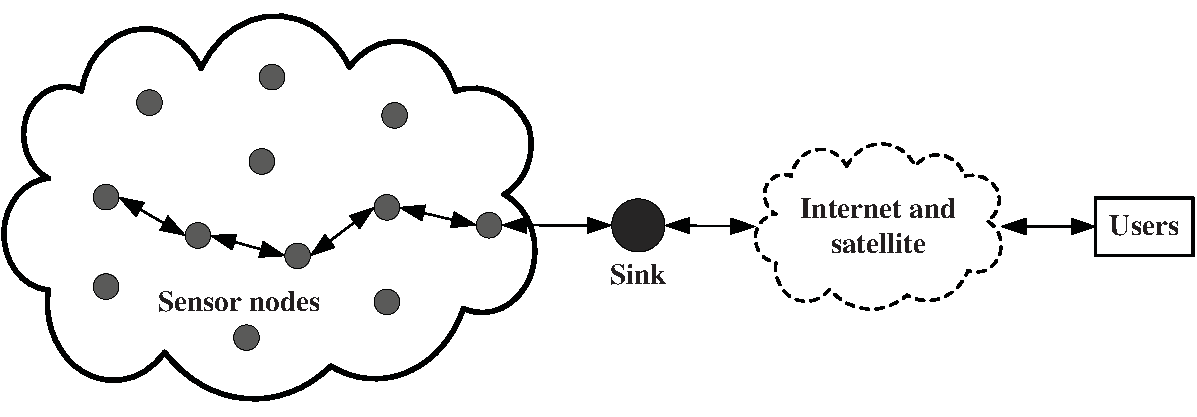
\includegraphics[width=0.75\textwidth]{fig101}
  \caption{典型的无线传感器网络体系结构图}
  \label{fig:101}
\end{figure}

无线传感网络的随机部署、环境复杂、无线自组织通信、感知能力等重要因素,使得其与传统的有线网络有着很大的不同;与其它形式的自组织网络相比,无线传感器网络一般具有更大的规模、更严格的资源限制、更少的基础设施支持等特点。因此,无线传感器网络在组织形式和性能评价等方面都有着自身鲜明的特点。

1. 资源受限

无线传感器网络具有的能量、通信能力、计算和存储能力都十分有限。受传感器节点的尺寸和造价的限制,节点的电源通常由电池提供,而部署的环境和规模使得通过更换电池来补充能量的方式代价过高。为了降低传感器节点的功耗、尺寸和造价,其通信距离和带宽均较小,所使用处理器的计算能力较弱,存储器容量也较小。

2. 应用相关

无线传感器网络是与应用密切相关的。虽然不同的应用可能存在一些共同的功能需求和解决方法,但是在传感器网络的研究中,必须充分考虑具体应用的特点和需求,进行定制的开发和优化,才能更好地克服资源受限的约束,设计出尽可能高效的系统。

3. 以数据为中心

无线传感器网络是一个以数据为中心的网络,网络的主要目标是将传感器节点感知到的数据完整地传递给最终用户。这和传统的以地址为中心的Internet有着明显的区别。传感器网络中不存在“端到端”的概念,而是由传感器节点和sink节点形成“多对一”(在多个sink节点的情况下也可以是“多对多”)的形式进行数据的扩散传播。

4. 大规模自组织网络

由于单个传感器节点的感知和通信范围均有限,要达到较大的覆盖范围就需要部署大量的节点。另外由于随机部署和环境干扰等因素,节点位置和节点间的连接关系不能预先精确设定。因此要求传感器节点具有自组织的能力,能够自动进行配置和管理,并通过节点间的分布式合作完成特定的任务。

5. 动态性强

传感器节点故障和失效、无线通信链路的不稳定性、传感器节点或者感知目标的移动性、新节点的加入等因素,以及拓扑控制、节点休眠调度等操作,都可能导致无线传感器网络的拓扑结构发生变化。因此无线传感器网络研究需要充分考虑其动态性强的特点。

6. 空间部署

在传统的有线网络的设计和实现中,通常很少涉及到节点具体的地理位置,而无线传感器网络却有着十分显著的空间部署特性。具体来讲,传感器节点的部署区域和地理位置会对网络功能的实现及其效率产生显著的影响。因此在无线传感器网络的路由、感知覆盖、数据收集和拓扑控制等关键协议和功能的设计中,需要充分考虑和利用网络的空间部署特性。

\subsection{研究现状}
早在1978年,美国DAPRA就在卡耐基-梅隆大学成立了分布式传感器网络小组。此后,DAPRA又联合美国自然科学基金委员会设立了多项传感器网络相关的研究项目。美国国防部和各军事部门也认为传感器网络未来将成为一种增强战场情报的感知能力、信息的综合和利用能力的重要手段,设立了一系列军事传感器网络研究项目。美国的很多大学都设立了专门的实验室和研究小组进行传感器网络的研究,比较著名的实验室和研究项目包括:加州大学伯克利分校的BWRC研究中心\upcite{BWRC}和WEBS研究项目\upcite{WEBS}、斯坦福大学的WSNL实验室\upcite{WSNL}、哈佛大学的Code Blue项目\upcite{CodeBlue}、加州大学洛杉矶分校的CENS实验室\upcite{CENS}和电子工程系的WINS项目\upcite{WINS}、卡内基梅隆大学的FireFly项目\upcite{FIREFLY}、南加州大学的RESL实验室\upcite{RESL}和信息科学研究所的SCADDS项目\upcite{SCADDS}、耶鲁大学的ENALAB实验室\upcite{ENALAB}、麻省理工学院的NMS项目\upcite{NMS}和AMPS项目\upcite{AMPS}、普渡大学的IDEAS实验室\upcite{IDEAS}、俄亥俄州立大学的ExScal项目\upcite{ExScal}、伊利诺斯大学香槟分校的INDEX研究组\upcite{INDEX}、科罗拉多大学波德分校的MANTIS研究项目\upcite{MANTIS}、乔治亚理工学院的BWN实验室\upcite{BWN}、纽约州立大学石溪分校的WINGS实验室\upcite{WINGS}。在工业界,IBM\upcite{IBM}、Microsoft\upcite{MICROSOFT}和Intel\upcite{INTEL}等公司也在从事传感器网络的相关研究。

国内也十分重视无线传感器网络的研究\upcite{Ni}。2006年初发布的《国家中长期科学与技术发展规划纲要》确定的信息技术的3个前沿方向中的两个与无线传感器网络研究直接相关。较早进行传感器网络研究的机构有中科院软件所\upcite{WSN_book}、计算所\upcite{cuili}、哈尔滨工业大学\upcite{lijianzhong}、清华大学\upcite{renfengyuan}、上海交通大学\upcite{cai}、北京大学\upcite{liuyongqiang}、以及南京大学\upcite{Wu}、国防科技大学\upcite{dong}、 浙江大学\upcite{zheng}、复旦大学\upcite{shen}、湖南大学\upcite{lin}、北京邮电大学\upcite{ma}、北京交通大学\upcite{renyan}等。2004年3月,中科院和香港科技大学成立了联合实验室,开展传感器网络的研究项目。2006年初,国家973计划成立了无线传感网络的基础理论及关键技术研究项目\upcite{Ni},包括香港科技大学、上海交通大学等在内的十多所重点高校联合展开对传感器网络各个层面的课题研究。国家自然科学基金和国家863高科技计划都设立了专项,资助传感器网络的研究。

迄今为止,已经有一些得到了实际应用的传感器硬件平台和系统软件被研制出来。比较有代表性的传感器节点包括加州大学伯克利分校和Crossbow公司联合开发的MICA系列节点\upcite{MICA}和Telos节点\upcite{Telos},Intel公司开发的Intel Mote节点\upcite{mote},BWRC研究中心开发的Pico Node节点\upcite{Pico},中科院计算所研制的EZ系列节点\upcite{EZ}。比较著名的操作系统包括加州大学伯克利分校开发的TinyOS系统\upcite{TinyOS},加州大学洛杉矶分校开发的SOS系统\upcite{SOS},浙江大学开发的SenSpire操作系统\upcite{SenSpire}等。而在实际应用方面,一系列具有一定规模的传感器网络系统也得到了部署和研究,典型的系统如表\ref{tab:101}所示\upcite{wangxiaoping}。
\begin{table}[htb]
  \centering
  \begin{minipage}[t]{0.95\textwidth} % 如果想在表格中使用脚注,minipage是个不错的办法
  \caption[典型的无线传感器网络系统]{典型的无线传感器网络系统}
  \label{tab:101}
    \begin{tabular}{cccccc}
      \toprule[1.5pt]
      {\hei 系统名称} & {\hei 研究机构} & {\hei 部署方式} & {\hei 部署方式} & {\hei 系统规模} & {\hei 设计寿命}\\ \midrule[1pt]
      VigilNet\upcite{VigilNet} & 弗吉尼亚大学 & 室外 & 电池 & 200 & 3-6个月 \\ \midrule[1pt]
      Motelab\upcite{Motelab} & 哈佛大学 & 室内 & 电源 & 190 & N/A \\ \midrule[1pt]
      SensorScope\upcite{SensorScope} & 洛桑理工学院 & 室外 & 电池 & 97 & 6个月 \\ \midrule[1pt]
      Trio\upcite{Trio} & 加州大学伯克利分校 & 室外 & 太阳能 & 557 & 4个月 \\ \midrule[1pt]
      GreenOrbs\upcite{GreenOrbs} & 香港科技大学 & 室外 & 电池 & 1000+ & 12个月 \\ \midrule[1pt]
      CitySee\upcite{CitySee} & 清华大学 & 室外 & 电池 & 2000+ & >24个月 \\
      \bottomrule[1.5pt]
    \end{tabular}
  \end{minipage}
\end{table}

\section{无线传感器网络拓扑压缩}
本节阐述无线传感器网络拓扑压缩技术的重要研究意义,并讨论从事该研究所面临的主要挑战。
\subsection{研究意义}
\begin{figure}[t]
  \centering
  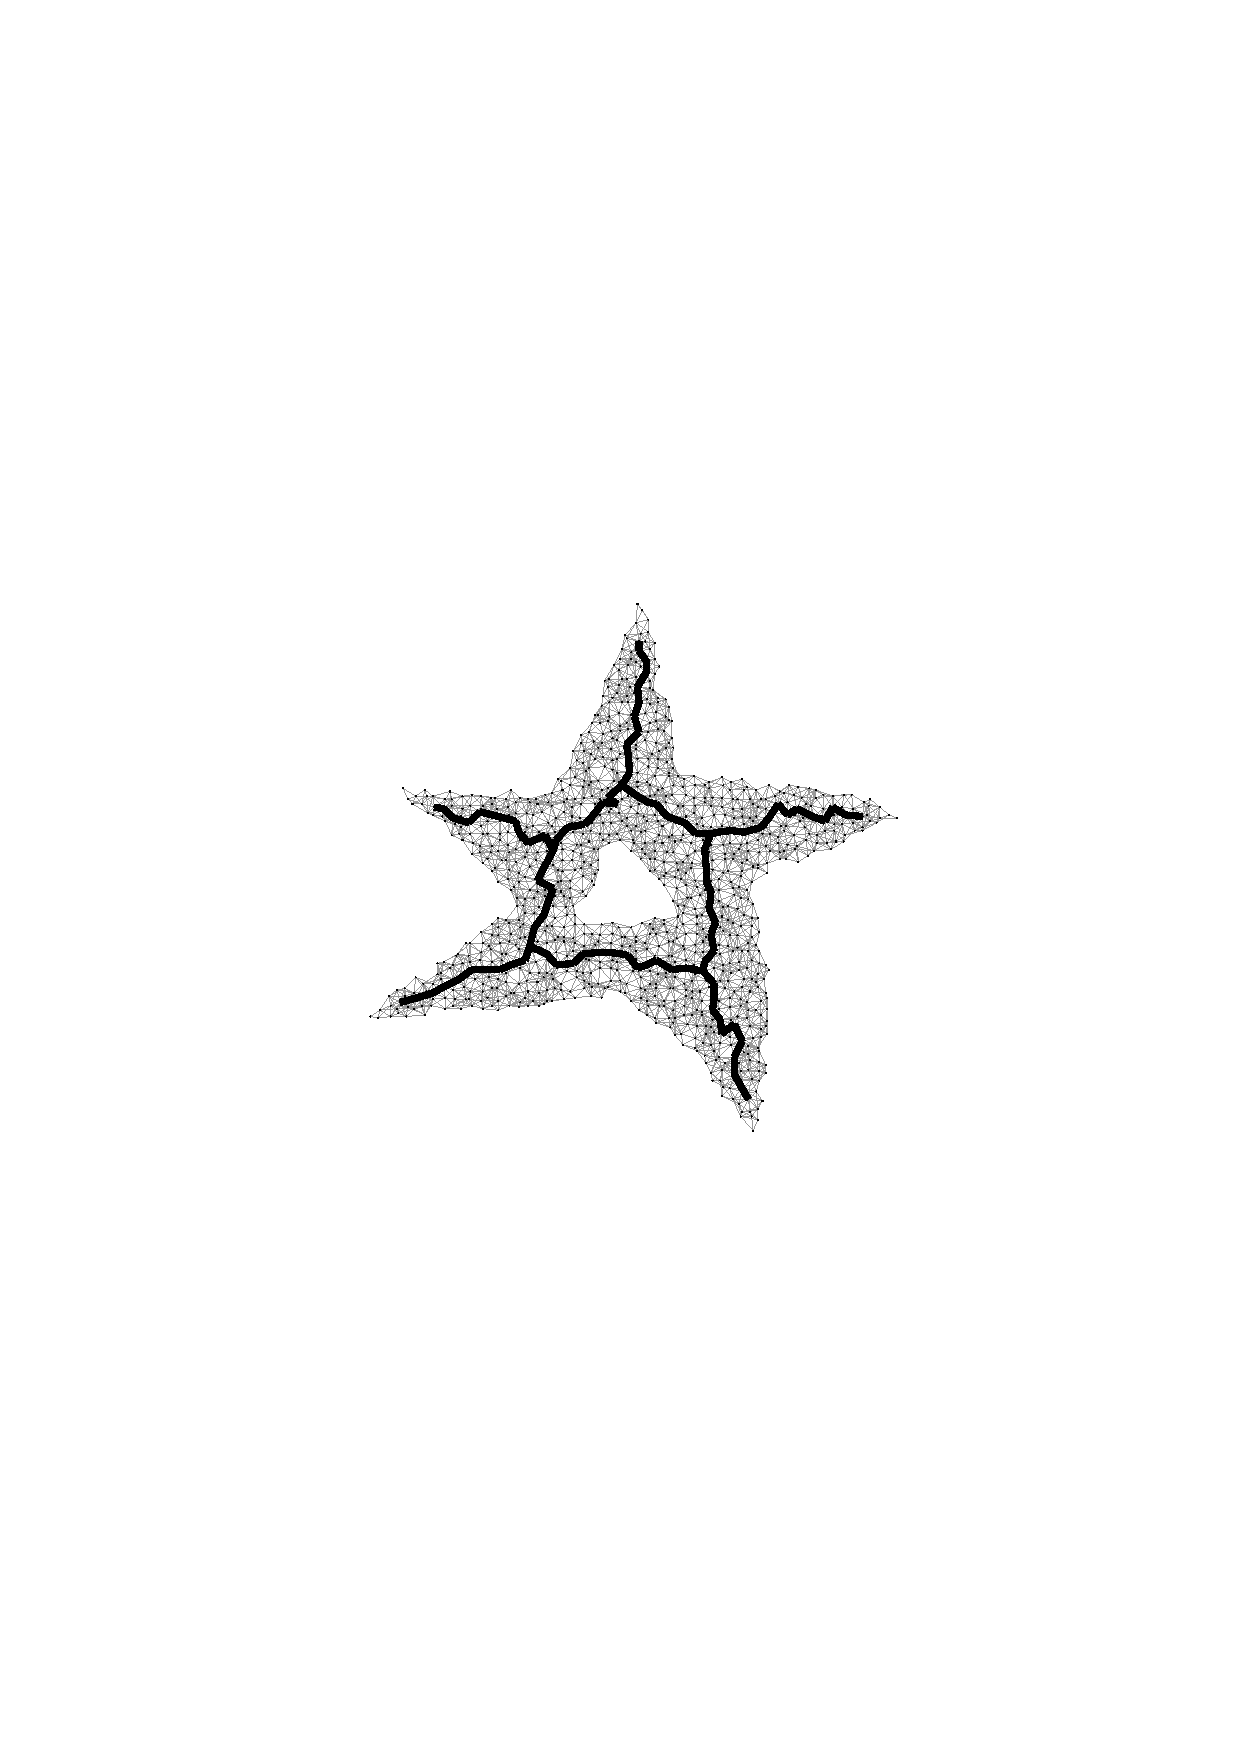
\includegraphics[width=0.5\textwidth]{fig102}
  \caption{拓扑骨干提取问题示例}
  \label{fig:102}
\end{figure}
无线传感器网络的拓扑结构是实现数据收集、处理、传输等重要网络功能的基础和保证,因此拓扑结构研究成为无线传感器网络中一项非常重要的研究内容。由于无线传感器网络与传统的有线和无线网络之间显著的区别,使得其拓扑结构的研究具有独特的限制和需求。特别是在大规模的网络系统中,对方法的简单性、可用性、可扩展性等提出了严格的要求。如果不加区分地对网络的完整拓扑信息进行研究和利用,往往难以得到高效的算法。而实际上,整个网络的关键拓扑特性往往可以通过部分的拓扑信息来描述,如网络边界、网络骨干、连通支配集等。这些特殊的拓扑结构对于设计高效的网络协议和算法具有至关重要的作用。因此,如何从完整的拓扑结构中识别或构建出这些特殊的拓扑信息就显得尤为重要,而这也正是拓扑压缩技术所要研究和解决的主要问题。简单来讲,拓扑压缩技术就是致力于从可用的全局或局部的网络拓扑信息中,提取出一部分具有特定结构和性质的拓扑子结构或其它形式的有效信息。例如在不依赖位置信息的拓扑骨干提取问题中,算法对给定的全局或局部的网络连通性信息进行压缩和化简,得到具有良好连通性和形状的骨干网络。如图\ref{fig:102}给出了拓扑骨干提取问题的一个示例,对于图示的星形网络,粗线表示利用拓扑压缩技术从网络中抽取出的拓扑骨干。利用拓扑压缩技术得到的这些拓扑子结构或其它信息又可以进一步的被利用来指导一系列网络功能或协议的设计和实现,从而改善网络的安全性、能力和效率等。目前已有的很多拓扑结构相关的研究内容实际上都属于拓扑压缩问题研究的范畴,如网络拓扑边界识别\upcite{bounary_infocom04,boundary_mobicom06,boundary_funke,boundary_funke2,boundary_kroller,boundary_ipsn08,boundary_mobihoc09}、 网络拓扑覆盖研究\upcite{cover_infocom01,cover_sensys03,cover_dongTC,cover_dongICDCS,cover_ipsn05,cover_mobihoc05,cover_mobihoc06,cover_infocom08,cover_mobicom09,cover_icnp07}、 虫洞拓扑的检测与识别\upcite{wormhole_cnds05,wormhole_icnp02,wormhole_infocom03,wormhole_wwcmc,wormhole_sasn03,wormhole_icnp06,wormhole_ndss04,wormhole_wise04,wormhole_infocom07,wormhole_mobihoc11,wormhole_ton,wormhole_icnp09,wormhole_icpads09}、
平面化拓扑的提取技术\upcite{planar_mobihoc01,planar_infocom02,planar_mobicom05,planar_nsdi05,planar_incocom07,planar_funke,planar_infocom08,planar_infocom11,planar_tmc}、 网络拓扑骨干的提取\upcite{skeleton_mobihoc05,skeleton_wn,skeleton_infocom09,skeleton_tpds10,skeleton_icdcs12,skeleton_icdcs122}等。本文在已有研究工作的基础上,进一步深入和系统地研究无线传感器网络拓扑压缩技术中的一些关键问题。

拓扑压缩技术对于无线传感器网络的研究具有重要的意义。由于大量的传感器节点通常被随机部署到目标区域内,各个节点在部署之初往往无法获得网络的全局信息,如网络区域的全局形状、节点自身在网络中所处的位置等。即使是在汇聚节点,实际上也难以很快获得全局的精确信息,如部署区域的几何形状、网络的重要拓扑特征(如网络边界、虫洞链路、网络骨干等)。这些信息对于网络功能的实现、网络安全性、网络协议的效率等,往往发挥着至关重要的作用。一些与部署相关的特征直接源自网络部署区域的几何特征,而要准确、完整的获得这些信息往往是十分困难的,尤其是在网络节点位置不可知或者是不精确的情况下尤其困难。传感器网络中的很多设计通常假设网络节点均匀随机地部署在没有洞的简单几何区域中,且节点的精确位置是可知的,但这些假设在实际的网络中是不现实的。拓扑压缩技术就是致力于在仅给定少量有效信息的情况下,如仅有局部或全局的网络连通性关系,或仅有全部或部分节点的不精确的位置信息,提取出系统或用户所需要的特定的拓扑特征。

可以用拓扑骨干提取技术来具体地说明拓扑压缩的研究意义。骨干提取问题源自计算机视觉\upcite{skeleton_vision}和计算机图形学\upcite{skeleton_graphics},并作为对研究对象几何特征的一种重要描述得到了广泛的研究。后来,骨干被引入到无线传感器网络的研究中,并被利用来改善很多网络协议和算法的性能,包括路由协议\upcite{skeleton_mobihoc05,skeleton_wn}、定位算法\upcite{localization_infocom08,skeleton_localization}、网络分区(segmentation)\upcite{segmentation_infocom07,segmentation_concel,segmentation_infocom12}、导航(navigation)\upcite{navigation_infocom06}等。例如,文献\upcite{skeleton_mobihoc05}提出了无线传感器网络中基于拓扑骨干的命名和路由方法,称为MAP,实现了局部的路由决策和良好的负载均衡性能。在骨干网络信息已知的基础上,MAP协议按照节点与骨干网络的相对位置(例如节点所处的骨干节点的最短路径树)和距离,对网络中的每个节点进行命名。然后,任意节点对之间按照其命名中的位置和距离信息,选择与骨干网络平行的路径作为路由路径。按照以上基本思想,MAP路由协议利用拓扑骨干有效地改善了算法的负载均衡性能。为了能够利用拓扑骨干的良好特性,设计拓扑骨干提取算法就成为重要的研究问题。拓扑压缩技术中一项重要的研究内容就是致力于从给定的网络连通性信息中,抽取出具有良好连通性和形状的拓扑骨干,进而利用拓扑骨干信息设计更加高效的网络协议和算法。因此,拓扑压缩技术对于以上协议和算法的实现至关重要。

下面再用虫洞拓扑的检测问题来说明拓扑压缩的意义。虫洞攻击是无线自组织和传感器网络中一种危害严重的攻击方式。在虫洞攻击中,攻击者在网络中相距较远的两个地点间设置恶意节点,并在恶意节点之间建立优质高速的虫洞链路,使得虫洞两端的节点误以为彼此距离很近,并通过虫洞链路直接传输数据包。通过发动虫洞攻击,攻击者能够显著地改变网络的拓扑结构,并借此发动多种危害严重的攻击。虫洞攻击的另外一个显著特点是攻击者可以在不破环任何合法节点或密码机制的情况下发动该攻击,因此传统的基于密码学的安全机制无法解决虫洞攻击\upcite{wormhole_infocom03}。为了解决虫洞攻击问题,研究者提出了大量的方案。早期的方法大部分是基于数据包的传输距离\upcite{wormhole_wwcmc}或传输时间\upcite{wormhole_infocom03,wormhole_sasn03}的失配来检测虫洞链路。但这些方法依赖于特殊的硬件设备或理想的网络假设,因此其可用性受到限制。为了提高虫洞攻击检测方法的可用性,研究者又提出了基于网络拓扑的检测方法\upcite{wormhole_infocom07,wormhole_mobihoc11,wormhole_ton,wormhole_icnp09,wormhole_icpads09}。这类方法通过从网络连通性信息中识别虫洞攻击造成的异常拓扑结构来检测虫洞。例如,文献\upcite{wormhole_mobihoc11}提出的方法基于如下观察来检测虫洞节点:正常节点的移除不会破坏其局部邻居子图的连通性,而虫洞节点的移除将使得其局部邻居子图被分割成两个独立的连通组件。接下来,方法通过提取出虫洞节点及虫洞链路构成的极大完全二部图来对其进行准确的定位。实际上,该类方法从本质上来看,正是利用了拓扑压缩技术从网络连通性信息中提取出虫洞拓扑结构。

另外,拓扑压缩技术还对其它很多的网络功能和协议具有重要的意义,如贪婪地理路由、感知覆盖、网络定位、数据聚合等。地理路由由于其简单性和低开销性得到了广泛的应用,但其固有的局部最小问题使得纯粹的贪婪地理路由协议无法提供传输保证。为了克服局部最小问题,研究者提出了大量的解决方案,其中最早也是应用最广泛的一种策略就是边缘路由\upcite{routing_mobicom00,routing_wn,routing_podc03,routing_cc,routing_dialm2002,routing_mobihoc03,routing_funke}。边缘路由中一个关键的步骤就是构建平面化连通子图。拓扑压缩技术就可以用来从给定的网络连通图中提取出平面化子图,从而为边缘路由提供基础。另外在感知覆盖方面,拓扑压缩技术可以用来构建满足特定覆盖质量要求的覆盖集合,如文献\upcite{cover_dongICDCS}提出的圈限覆盖方法,通过从网络中选取尽量少的节点来满足期望的圈限覆盖(即覆盖空洞的直径不大于给定的门限值),在满足覆盖质量要求的基础上使其它节点进入休眠以节约能量。拓扑压缩技术还可以用来识别网络边界,进而辅助定位和追踪特定事件\upcite{tracking},为测距无关的节点定位\upcite{localization_mobicom07,localization_infocom08}、网络分割\upcite{shapesegmentation} 等重要的网络服务提供基础等。此外,拓扑压缩技术还可以用来从网络中提取出具有特定属性的节点集合和拓扑结构,如利用连通支配集构建骨干网络\upcite{cds_dingling,cds_du},并为路由协议、数据聚合等很多重要网络功能的设计和实现提供指导。综上所述,拓扑压缩技术对无线传感器网络中大量的重要网络功能的实现和高效网络协议的设计具有重要的指导作用,是无线传感器网络中一项核心研究内容。

\subsection{研究挑战}
在无线传感器网络中,大量能力受限的传感器节点被随机部署在监测区域内,以无线自组织的方式形成网络,协作地完成数据的收集、处理和传输任务。与传统的有线网络和其它形式的自组织网络相比,无线传感器网络具有更大的网络规模、更严格的资源限制、更少的基础设施支持,而且往往部署在环境复杂、人力无法到达的区域。因此,无线传感器网络的研究面临着独特的限制、需求以及挑战。具体来讲,由于无线传感器网络具有显著的空间部署特征,其网络拓扑受到部署区域的几何形状的约束。因此,节点的位置信息对传感器网络拓扑结构的相关研究有着根本的影响。目前,无线传感器网络中与拓扑结构相关的大部分研究工作均基于已知节点精确位置信息这一理想假设,进而简化了算法设计的难度。但是同时,对于精确位置信息的依赖也严格限制了这些算法的实际可用性。

在实际的大规模无线传感器网络中,获取节点的精确位置信息往往十分困难,甚至是无法实现的。首先,传感器网络通常随机部署在监测区域,例如通过飞机投放等方式,因此节点的位置信息往往无法通过预先设定的方式来获得。其次,传感器网络往往部署在恶劣或者敌对环境中,因此通过手动配置每个节点的位置信息也是不现实的。同时传感器网络的大规模使得人工配置需要很长的部署和启动时间,也将导致失去自组织网络的优势。因此获取网络位置信息主要依赖网络定位服务。定位服务的实现主要有两种途径:第一种是通过在每个节点上装备GPS设备;第二种则是在少量的节点上装备GPS设备,其余节点通过网络化的定位算法计算位置。对于第一种途径,由于受到传感器节点的尺寸、造价、能耗等因素的限制,要实现在每个节点上都装备GPS节点是不现实的,且GPS设备仅适用于无遮挡的室外环境。第二种途径存在大量的研究成果,如基于测距的定位\upcite{localization_infocom00,localization_mobicom00,localization_cn}、基于夹角的定位\upcite{localization_angle}等,但是这些算法仍存在很多的限制。首先,各种定位技术存在明显的定位误差\upcite{localization_error1,localization_error2}。这是由于各种测距手段均存在误差,因此节点的定位结果也相应地存在误差。而且由于误差的累积和其它不确定因素的增长,最终可能会导致位置误差非常大。其次,即使测距信息是精确的,网络仍有可能是不可定位的。这种情况可能由两种因素造成:第一种是由于网络测距图本身在理论上就是不可定位的,在这方面有大量的有关定位理论的研究成果\upcite{localization_infocom04};第二种是即使网络在理论上是可定位的,计算这些可定位节点的具体位置的问题仍然是NP难问题\upcite{localization_TMC}。

为了改善系统在位置信息不可用或不精确情况下的可用性,研究者提出了不依赖位置信息的拓扑结构研究方法。这类方法以网络连通图为研究对象,利用通讯图模型和一定的图理论工具对网络拓扑结构进行研究。但是,这类方法的研究仍然面临着很多的挑战。

首先是资源受限,对算法的复杂度提出了严格的要求。由于传感器节点的计算、存储能力都比较弱,使得单个节点无法完成复杂的计算任务,因此对算法的计算复杂度提出了严格的要求;另外由于节点的能量约束,要求节点间的通信开销尽可能的低,从而对算法的消息复杂度提出了严格的要求。

其次是有效信息受限,使得算法的设计难度较高。在没有节点位置信息的情况下,算法设计可以利用的有效信息主要是网络连通性信息及通讯图模型(如单位圆盘图模型)。而通讯图模型实际上反映的只是连通图的局部特征,难以处理很多涉及到网络全局拓扑结构的问题。例如仅已知网络连通图符合单位圆盘图模型,要计算全网的有效嵌入(即节点可能的位置)是NP难的\upcite{embedding_np}。因此在不依赖位置信息的拓扑结构研究中,必须深入分析网络连通性信息,结合所研究的具体拓扑问题的特点和相关约束及假设,挖掘出能够反映全局性质的结构和有效信息。

第三是在位置信息不可用的情况下,要保持较低的几何失真率非常困难。在进行拓扑结构相关研究时,为了提高算法和位于其上层的各项协议的可靠性和效率,要求在算法的执行过程和结果中始终尽量地保持网络的几何特征(如部署区域的几何形状、节点间的位置关系),即保持较低的几何失真率。而在仅利用连通性信息的情况下,特别是在仅局部连通性信息可用时,要实现这一目标非常困难。因此,保持较低的几何失真率是无线传感器网络拓扑压缩技术研究面临的关键挑战。

第四是研究方法和理论工具受限。由于没有节点位置信息,传统的计算几何的方法无法使用;单纯的图理论方法虽然适用于仅有连通性信息的情况,但缺乏对网络几何特性的充分利用。近年来,代数拓扑学被引入到无线传感器网络拓扑结构研究中,并取得了一定的成果\upcite{boundary_mobicom06,cover_ipsn05,wormhole_ton,wormhole_icnp09,cover_homology}。代数拓扑学能够很好地反映网络连通图的拓扑性质,同时与网络的几何实现紧密关联,因此适用于传感器网络拓扑结构的研究。但是代数拓扑学方法往往依赖全局的连通关系和集中式的计算,这在大规模无线传感器网络中是难以实现的。另外,仅利用代数拓扑学工具往往无法准确地反映网络的几何特性。因此,如何结合几何、图论、拓扑学的技术,针对特定的拓扑问题建立有效的拓扑分析工具,并设计高效的分布式算法,是拓扑压缩技术研究的难点之一。
\section{研究内容与创新点}
拓扑结构一直是无线传感器网络中一项重要的研究内容。本文系统地研究了无线传感器网络拓扑压缩技术中的一些重要问题。图\ref{fig:103}显示了本文的研究内容及其相互关系。本文首先在第三章研究了拓扑骨干的提取问题,提出了不依赖位置信息的拓扑骨干提取算法,通过对网络连通图进行压缩简化,提取出具有连通性保证、符合网络部署区域几何特征的骨干网络;第四章研究了虫洞拓扑检测问题,深入分析虫洞攻击对网络全局的拓扑结构造成的本质影响,提出了基于网络平面化的虫洞检测方法,能够准确地检测和定位虫洞节点和虫洞链路;第五章首次提出并系统地研究无线传感器网络的路由路径记录问题,提出了高效的路由路径压缩和恢复方法,能够有效地记录网络中所有数据包的精确传输路径,从而显著地改善网络内部状态的可见性;第六章研究了拓扑压缩技术在地理路由协议设计中的应用,利用已有的细粒度的拓扑平面化算法,设计了一种高效的、细粒度的、不依赖精确位置信息的贪婪地理路由协议。以上各个问题都是无线传感器网络中的重要研究内容,也获得了广泛的关注和深入的研究。从整体上来看,第三、四章研究了网络骨干、虫洞拓扑这两种网络连通性拓扑结构,分别可以看作连通性拓扑的构建和识别问题;第五、六章研究了路由路径、贪婪路由这两种路由拓扑问题,分别可以看作路由拓扑的记录(或识别)和构建问题。本文以改善方法的可用性和效能为目标,对以上各个问题展开深入的研究,针对已有的方法中存在的不足,提出了相应的解决方案。本文在研究过程中,将尽量不依赖位置信息(或仅有不精确的位置信息),同时又能够保证较低的几何失真率作为贯穿始终的算法设计标准。具体来讲,较低的几何失真率在拓扑骨干提取问题中体现为提取出严格符合网络部署区域的几何形状的拓扑骨干,在虫洞拓扑识别问题中体现为较高的虫洞检测准确率,在路由路径记录问题中体现为以较低的代价记录数据包的完整路径信息,在地理路由协议的设计中体现为较低的路径失真率。
\begin{figure}[t] % use float package if you want it here
  \centering
  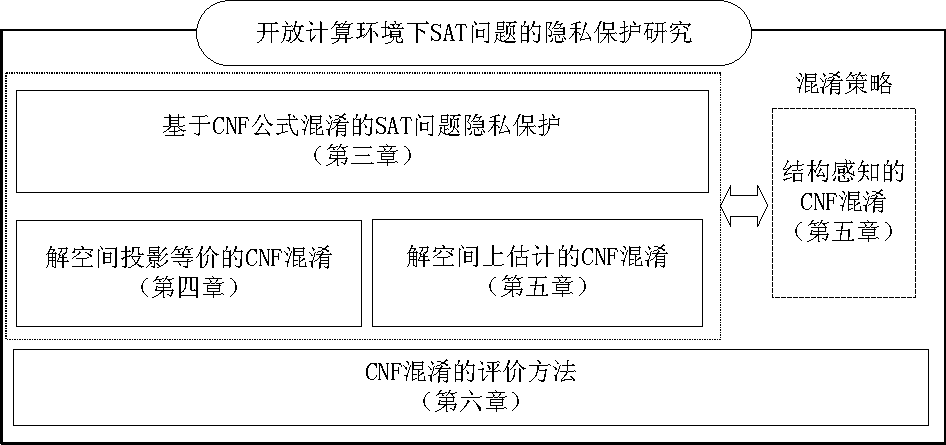
\includegraphics[width=0.8\textwidth]{fig103}
  \caption{本文研究内容}
  \label{fig:103}
\end{figure}

本文受国家自然科学基金项目“无线传感器网络不依赖位置信息的拓扑识别与构建技术研究”(项目编号61272482)的支持,主要贡献和创新点如下:

1. 不依赖位置关系的拓扑骨干提取。

不依赖位置信息的拓扑骨干识别是拓扑压缩技术的重要研究内容。现有的方法\upcite{skeleton_mobihoc05,skeleton_wn,skeleton_infocom09,skeleton_tpds10,skeleton_icdcs12,skeleton_icdcs122}往往基于较强的网络假设,如均匀、密集部署的网络条件等,或无法给出可证明的、确定性的结果。这些因素显著地限制了方法的性能和应用范围。本文致力于设计不依赖位置关系,具有良好鲁棒性的拓扑骨干提取方法。算法利用了仅依赖局部连通性信息的基于MDS的边界识别算法,提出了骨干带网络构建方法以及高效的图变换工具HPT,并设计了一种灵活有效的骨干叶节点判定方法。算法能够适用于各种不同形状的网络,提取出具有良好连通性和形状的拓扑骨干,且对多种关键的网络参数具有良好的鲁棒性。本文从理论上证明了算法的正确性并通过大量的仿真实验验证了算法的性能。

2. 不依赖位置信息的虫洞拓扑识别。

在研究了拓扑骨干这一低维拓扑特征的提取之后,本文进一步研究网络由于受到虫洞攻击而产生的异常的高维拓扑特征。现有的大部分虫洞检测方法依赖于专业的硬件设备或理想的网络假设\upcite{wormhole_cnds05,wormhole_icnp02,wormhole_infocom03,wormhole_wwcmc,wormhole_sasn03,wormhole_ndss04},从而在很大程度上限制了这些方法的可用性。为了改善方法的可用性,研究者提出了基于连通性信息的虫洞检测方法\upcite{wormhole_infocom07,wormhole_mobihoc11,wormhole_ton,wormhole_icnp09,wormhole_icpads09}。这类检测方法大致分为两类:第一类方法直接在离散域捕获局部的虫洞症状,这类方法比较简单,但往往不够准确,如在稀疏网络中的误报率较高;第二类方法在连续域分析全局的虫洞拓扑症状,这类方法准确率较高,但是在将连续域中的虫洞症状转换成离散域的检测算法时容易产生失真。针对现有方法的局限性,本文深入挖掘虫洞攻击对全局的拓扑结构造成的本质影响,发现一种虫洞攻击的新症状,即虫洞攻击对网络平面化造成的影响,并提出了一种仅利用局部连通性信息的虫洞检测方法,称为WormPlanar。WormPlanar首次实现了直接从离散域捕获虫洞造成的全局拓扑症状。本文从理论上充分证明了算法的正确性,并通过大量的仿真实验验证了方法的有效性和性能。

3. 轻量级的路由路径记录方法。

在大规模无线传感器网络中,路由路径记录对可靠的数据传输和细粒度的网络管理具有重要的作用。但严格受限的资源使得设计一种轻量级、实际可用的路由路径记录方法非常具有挑战性。已有的大量研究工作,如网络诊断和调试等\upcite{diagnosis_pad,diagnosis_sympathy,diagnosis_tolle,diagnosis_woo},虽然在一定程度上利用了数据包的路由路径信息,但是均没能实现完整地记录每个数据包的精确路径信息。本文首次正式地提出并系统地研究无线传感器网络的路由路径记录问题,提出了一种轻量级的、在实际的大规模网络中可用的路由路径压缩和恢复方法,称为PathZip。本文设计了基于哈希的路径压缩和恢复机制,将大部分的计算和存储开销从传感器节点转移至基站。另外,PathZip利用了分别基于拓扑和基于几何的技术来降低算法的开销。本文通过理论证明和大量的仿真实验验证了算法的有效性和性能,结果显示PathZip能够实时地记录每个数据包的完整传输路径,且计算复杂度和存储开销均低于相关的数据压缩算法。

4. 不精确位置信息下的层次式贪婪地理路由。

贪婪地理路由协议由于其简单性和低开销得到了广泛的应用,但其固有的局部最小问题使得纯粹的贪婪地理路由方法无法提供传输保证。为了克服局部最小问题,研究者进行了大量的工作\upcite{routing_mobicom00,routing_wn,routing_podc03,routing_cc,routing_dialm2002,routing_mobihoc03,routing_funke}。这些方法具有各自的优势和适用范围,在一定的假设条件下有效地克服了局部最小问题。本文结合已有的各类方法的优势,提出了一种细粒度的层次式贪婪地理路由方法,称为FLYER。FLYER不依赖精确的位置信息或全局的状态信息,在节点位置误差率不超过一定上限值时具有传输保证。FLYER方法以完全分布式的方法运行,且具有较低的计算和存储开销。本文从理论上证明了FLYER方法的有效性,并通过大量的仿真实验验证了方法的性能,结果显示在贪婪路由成功率、路径长度、负载均衡性等各项性能指标上,FLYER均优于之前的设计。
\section{论文组织结构}
论文共分七章,组织结构如下:

第一章为绪论,介绍传感器网络的基本概念、特点、应用以及研究现状。分析无线传感器网络拓扑压缩技术的研究意义和挑战,并简述本文的研究内容和组织结构。

第二章为相关研究,对拓扑结构及拓扑压缩的相关问题进行了系统和全面的介绍,分析了现有工作的特点和适用性。

第三章研究不依赖位置信息的拓扑骨干提取问题。提出了仅利用局部连通性信息,具有良好鲁棒性的分布式拓扑骨干提取算法。

第四章研究不依赖位置信息的虫洞拓扑识别问题。深入地分析了虫洞对网络拓扑结构造成的根本影响,提出了仅利用局部连通性信息的分布式虫洞检测方法。

第五章研究路由路径记录问题。巧妙地提出了基于哈希的路由路径压缩和恢复方法,并设计了分别基于拓扑和基于几何的策略来降低算法的开销。

第六章研究贪婪地理路由问题。利用层次式路由设计的思想和灵活的拓扑平面化算法,设计了不依赖精确位置信息、具有良好可用性和可扩展性的高效的贪婪地理路由方法。

第七章总结全文并展望未来的工作。

最后是致谢、博士期间撰写的论文、参加的科研工作以及参考文献。
